\documentclass[
	11pt
] {article}

\usepackage[
	a4paper,
	left=3cm,
	right=2cm,
	top=2cm,
	bottom=2cm,
	headheight=1cm
] {geometry} %for setting margin

\usepackage{fancyhdr} %for header and footers
\usepackage{parskip} %for leaving some space after paragraphs


% Math
\usepackage{mathtools} %helps to number equations
\usepackage{siunitx} % Units of measurement


% For graphs and advanced diagrams
\usepackage{tikz} %the drawing library
\usetikzlibrary{positioning} %some auxilary to the drawing library
\usetikzlibrary{math} %helps to define variables in the tikz

\usepackage{authblk} %authors and their affiliations

% Basic graphics
\usepackage{float} %to force the figure to be in a place among the text
\usepackage{graphicx} %for include graphics
\usepackage{caption} %better referencing to labels
\usepackage{subcaption}  %helps with multiple pictures in a figure


% Language and Font package: COMMENT THESE FOR ENGLISH ONLY
\usepackage[T2A]{fontenc} %[RUS] loads cyrillic characters
\usepackage[russian, english]{babel} %[RUS] changes date heading 'abstract' to Russian
\usepackage[utf8]{inputenc} %[RUS] to force utf-8 encoding


%-----------------------------------------------------------------------

%\renewcommand\thesubfigure{\asbuk{subfigure}} %[RUS] for renaming subfigures to russian
%\sisetup{output-decimal-marker = {,}} %[RUS] changes all ordinary decimal separator to rassiky commas
\pagestyle{fancy}
\graphicspath{{figures/}}



\newcommand\titlecustom{The rules of Living}
\author[]{Wernher von Braun}
\title{\titlecustom}
\fancyhead{}
\fancyhead[L]{}
\fancyhead[C]{\titlecustom}
\fancyhead[R]{\the\year}



\begin{document}


\maketitle


\tableofcontents


%~ \section{Template}
	%~ \subsection{Equations}
		%~ \begin{equation} \label{eq:defaut-darcy-law}
			%~ Q = \frac{k}{\mu} \Delta P
		%~ \end{equation}

		%~ This is a sample reference to equation \ref{eq:defaut-darcy-law}.

	%~ \subsection{Table}
		%~ \begin{table}[H]
			%~ \centering
			%~ \caption{Sample caption of the table}
			%~ \label{table:default-1}
			%~ \begin{tabular}{| c | c | c |} % or ccS
				%~ \hline
				%~ Surface & Area (\si{\metre\squared}) & {Coefficient of absorption}\\
				%~ \hline
				%~ ceiling & 140 & 0.8 \\
				%~ walls & 260 & 0.03 \\
				%~ floor & 140 & 0.06 \\
				%~ \hline
			%~ \end{tabular}
		%~ \end{table}

		%~ This is a sample reference to table \ref{table:default-1}.

	%~ \subsection{Referencing subsections target 1} \label{subsec:default-part-1}
		%~ Some default text for target sub section 1.

	%~ \subsection{Referencing subsections target 2}  \label{subsec:default-part-2}
		%~ Some default text for target sub section 2.

	%~ \subsection{Referencing sections and sub sections}
		%~ This is a reference to sections or subsections \ref{subsec:default-part-1} and \ref{subsec:default-part-1}.

	%~ \subsection{Single Figure}
		%~ \begin{figure}[H]
			%~ \centering
			%~ 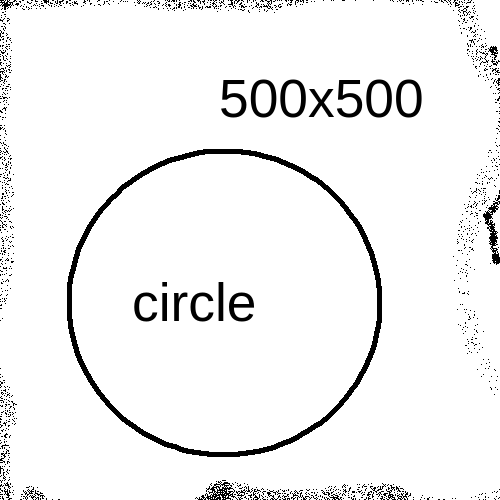
\includegraphics[width=0.5\textwidth]{fig-default-02}
			%~ \caption{A single figure}
			%~ \label{fig:default-single-figure}
		%~ \end{figure}

		%~ This is a sample reference to the figure \ref{fig:default-single-figure}.

	%~ \subsection{Figure with subfigures}

		%~ % H: forces to be in the place
		%~ % h: tries to put on place
		%~ % t: on top of page
		%~ % ht: here or top of next available space
		%~ \begin{figure}[H]
			%~ \centering
			%~ \begin{subfigure}[b]{0.49\textwidth}
				%~ \centering
				%~ 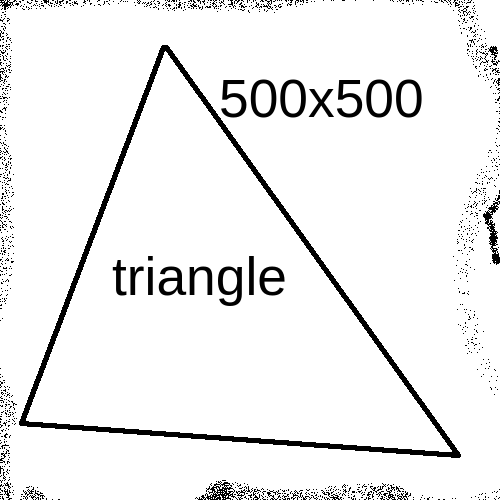
\includegraphics[width=\textwidth]{fig-default-01}
				%~ \caption{Label of subfig-a $S = \pi r^2$.}
				%~ \label{subfig:default-a}
			%~ \end{subfigure}
			%~ \hfill
			%~ \begin{subfigure}[b]{0.49\textwidth}
				%~ \centering
				%~ 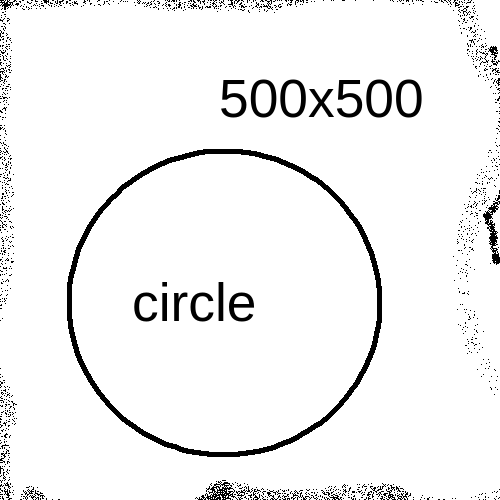
\includegraphics[width=\textwidth]{fig-default-02}
				%~ \caption{Label of subfig-b $S = a + b + c$.}
				%~ \label{subfig:default-b}
			%~ \end{subfigure}
			%~ \caption{Caption of both the figures}
			%~ \label{fig:default-label-figure-two-shapes}
		%~ \end{figure}

		%~ Figure \ref{fig:default-label-figure-two-shapes} contains \ref{subfig:default-a} and \ref{subfig:default-b}.

	%~ \subsection{Figure Drawing on Latex}
		%~ \begin{figure}[H]
			%~ \centering
			%~ \begin{tikzpicture}
				%~ \draw[blue, thick] (0,0) rectangle (3,2);
				%~ \draw[orange, thick] (4,0) -- (6,0) -- (5.7,2) -- cycle;
			%~ \end{tikzpicture}
			%~ \caption{Tikz figure}
		%~ \end{figure}

	%~ \subsection{Citation}
		%~ This is an example of citation \cite{ramstad2019pore}.

\bibliographystyle{plain.bst}
\bibliography{reference}
\end{document}
